\documentclass[11pt,a4paper]{article}

\usepackage[margin=2.3cm]{geometry}
\usepackage{graphicx}
\usepackage{booktabs}
\usepackage{tabularx}
\usepackage{xcolor}
\usepackage{listings}
\usepackage{siunitx}
\usepackage{enumitem}
\usepackage[colorlinks=true,linkcolor=blue!50!black,urlcolor=blue!50!black,citecolor=blue!50!black]{hyperref}

\lstset{basicstyle=\ttfamily\small,columns=fullflexible,breaklines=true,
        frame=single,framerule=0.3pt,rulecolor=\color{black!30},backgroundcolor=\color{black!3}}

\newcommand{\pr}[1]{\href{https://github.com/ucgmsim/sw4/pull/#1}{\#{#1}}}
\newcommand{\code}[1]{\texttt{#1}}

\title{QuakeCore 2026: SW4 Performance Consultancy\\[0.3em]
       \large Progress report, 22 September -- 29 October 2026}
\author{Alexander Pletzer, Geoffrey Weal (REANNZ) and\\
        Jake Faulkner (QuakeCore/University of Canterbury)}
\date{29 October 2026}

\begin{document}
\maketitle

\begin{abstract}
This report summarises the work carried out for QuakeCore under the REANNZ
consultancy ``QuakeCore 2026'' since its start on 22 September 2026. The
consultancy targets the single-precision port of the seismic wave propagation
code SW4 (\href{https://github.com/ucgmsim/sw4}{\code{ucgmsim/sw4}}, branch
\code{single\_precision}). Over five weeks we validated the single-precision
port, established the best compiler, build and runtime configuration on
Mahuika and Cascade, built in-code profiling, and removed several performance
bottlenecks. Sixteen pull requests have been merged upstream. The combined
changes roughly halve the time to solution on QuakeCore's production
rupture-source cases, and SW4 weak-scales with an efficiency of
1.10 from 1 to 8 Cascade nodes (1536 cores).
\end{abstract}

\section{Scope and tasks}

The consultancy was set up with the following tasks:
\begin{enumerate}[itemsep=0pt]
  \item Confirm the observed performance of SW4 in single versus double
        precision and find the performance hotspots.
  \item Review the single-precision port and validate that it is technically
        sound and suitable for production use.
  \item Work with the project researchers to profile SW4, identify bottlenecks,
        and investigate why single-precision runs are slower than expected.
  \item Agree on a performance improvement strategy, implement it, test the
        changes and report the new performance.
  \item Evaluate code changes, build options and runtime configurations to
        identify the optimal settings for SW4 on HPC systems.
\end{enumerate}
Work was coordinated between REANNZ and QuakeCore in weekly meetings. All code
changes were submitted as pull requests against \code{ucgmsim/sw4}
\code{single\_precision}, reviewed and checked by the project's CI
(regression tests and \code{clang-tidy}).

\section{Summary of accomplishments}

\begin{itemize}[itemsep=2pt]
  \item \textbf{Single-precision port validated.} The port now builds with
        Clang and GCC via a CMake switch (\code{-DUSE\_DOUBLE=OFF}); test
        tolerances were adjusted so the test suite passes in single precision.
        Single precision is 1.3--1.9$\times$ faster than double, with errors
        that stay at the level of the discretisation error except near
        mesh-refinement interfaces (Section~\ref{sec:validation}).
  \item \textbf{Best build configuration found.} On Mahuika Genoa nodes the
        classic Intel compiler with AVX-512 (\code{-march=icelake-server
        -qoverride-limits -qopt-zmm-usage=high}) is fastest, 27--29\% ahead of
        GCC~15 and 2--5$\times$ ahead of the previous \code{gimkl}/AOCC builds
        (Section~\ref{sec:build}).
  \item \textbf{Built-in profiling.} SW4 now reports hierarchical region
        timers with MPI and OpenMP (OMPT) costs at the end of every run, with
        no need for external tools such as TAU (Section~\ref{sec:timers}).
  \item \textbf{Kernel and algorithmic speedups.} A source time-function
        cache, constant-bound loops in the upper SBP closure, a reordered
        \code{Sarray::assign}, halo-only zeroing and $j$-tiling of the
        Cartesian RHS kernels. Individually these give between a few percent
        and 1.8$\times$; on a 30-event Darfield production campaign the
        run time fell from about 3~h to 1.5~h (Section~\ref{sec:opt}).
  \item \textbf{Bugs fixed.} Chunked float I/O in \code{Parallel\_IO},
        a missing reduction in the interface Jacobi solver, and several
        build portability problems (Section~\ref{sec:bugs}).
  \item \textbf{Runtime configuration and scaling on Cascade.} Pinning one
        MPI rank per 8-core CCD with 8 OpenMP threads is optimal;
        hyperthreading costs 31\%. Weak-scaling efficiency is 1.10 at 8 nodes
        (Section~\ref{sec:scaling}).
\end{itemize}

\section{Validation of the single-precision port}
\label{sec:validation}

The \code{single\_precision} branch did not compile with Clang~21 on macOS
because of mixed float/double arithmetic: calls such as \code{pow(x,2)} promote
float arguments to double, creating ambiguous overloads and, more importantly,
silent conversions in inner loops. These were fixed (PR~\pr{2}) and a CMake
single/double switch was added. The test tolerances were relaxed where the
differences between single and double were consistent with round-off.

Twilight-zone (manufactured solution) and Lamb problem tests show no visible
differences between single and double for tests without mesh refinement
(\code{flat-twi-1}, \code{lamb-1}, \code{tw-att-1}). With mesh refinement
(\code{refine-att-1}, \code{refine-el-1}) the single-precision error is
noticeably larger (Fig.~\ref{fig:refine}). The parts of the code that require
double precision (the interface Jacobi iteration and mass-block inversion) were
identified as candidates to remain in double.

\begin{figure}[ht]
  \centering
  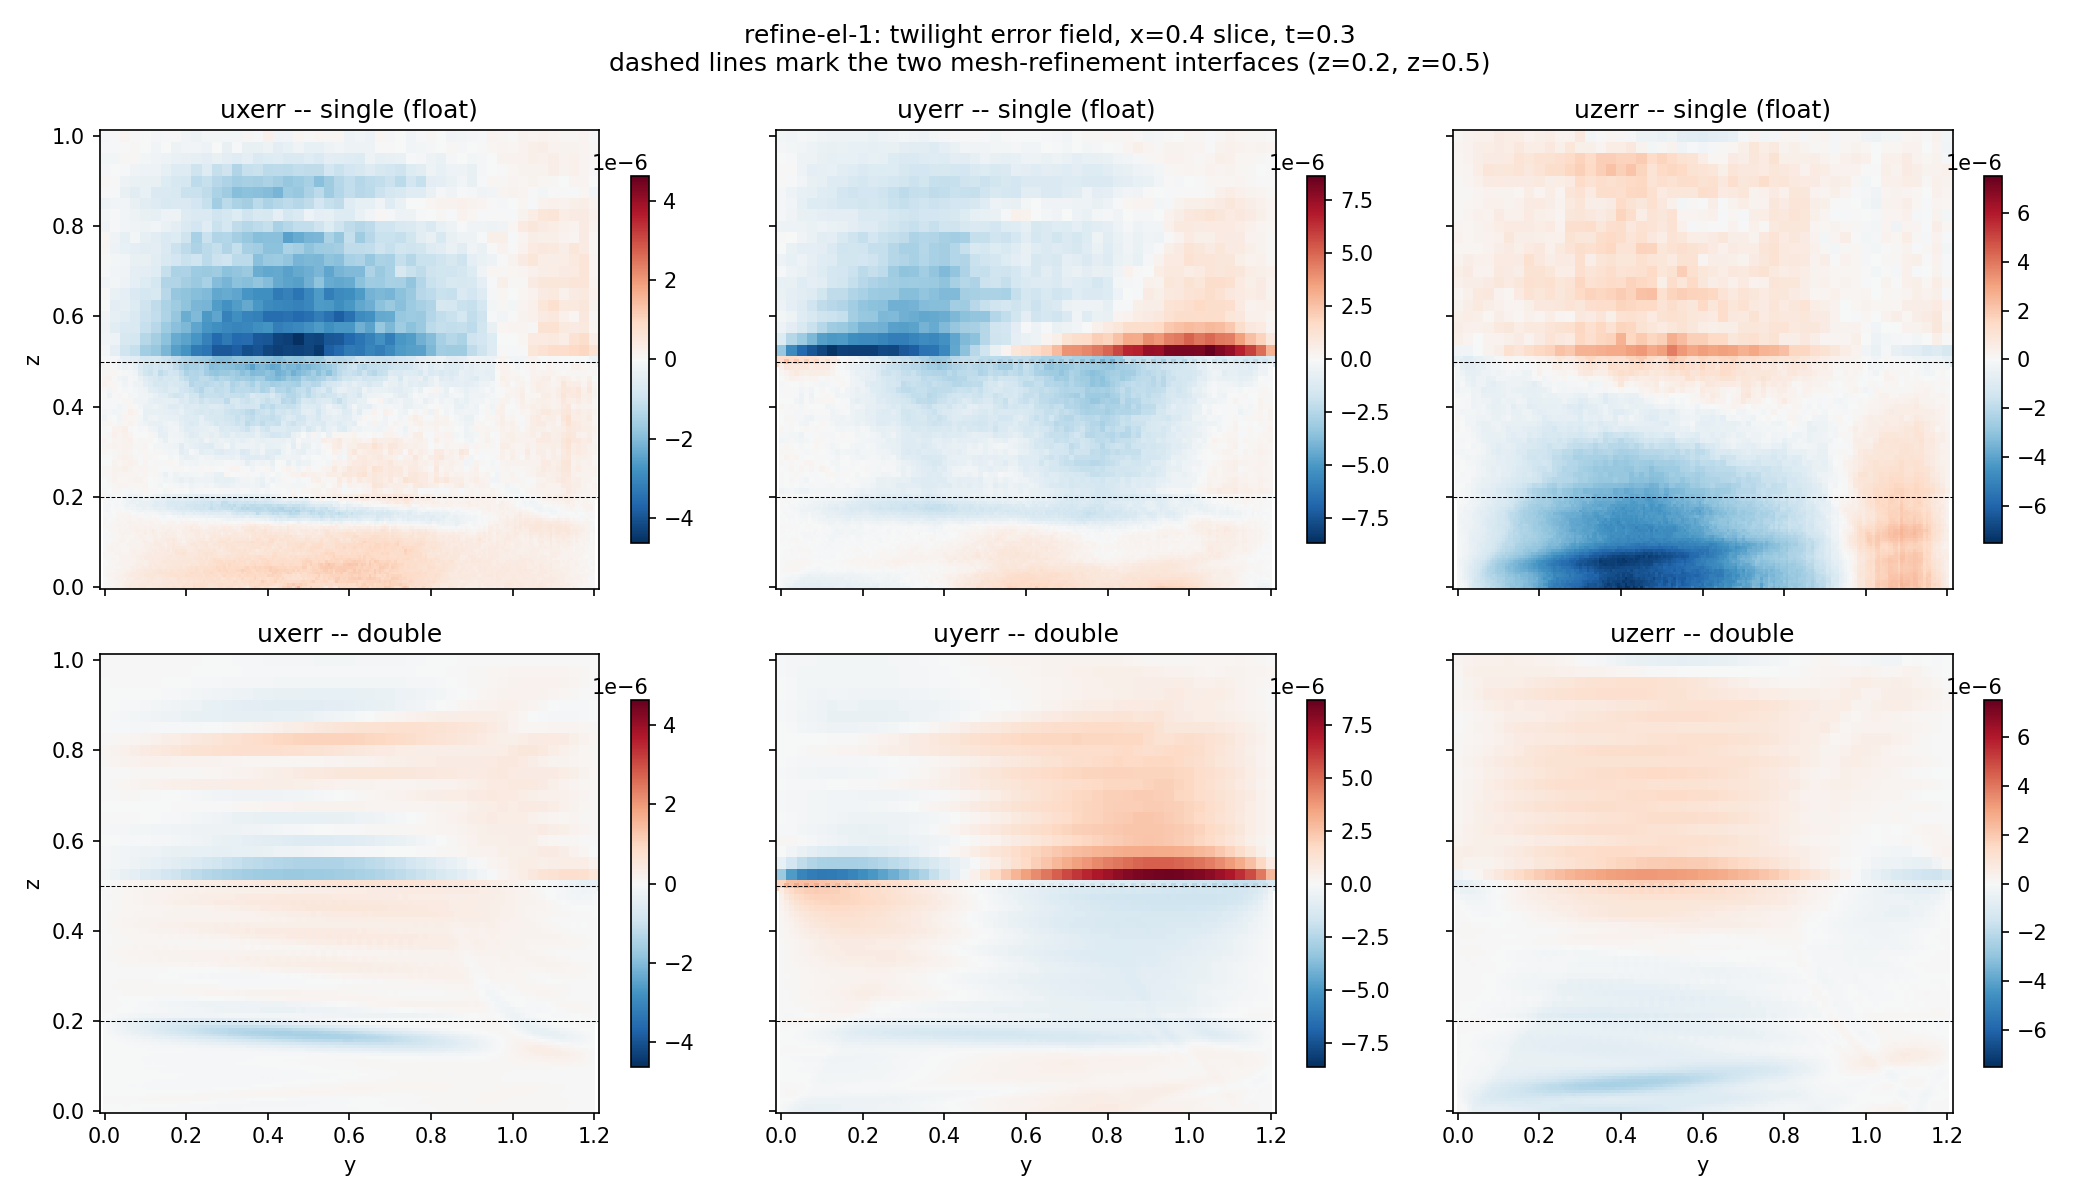
\includegraphics[width=\textwidth]{figures/refine_el1_float_vs_double.png}
  \caption{Twilight error field for \code{refine-el-1} on the slice $x=0.4$ at
    $t=0.3$, single (top) versus double (bottom) precision. The dashed lines
    mark the two mesh-refinement interfaces. The single-precision error has the
    same amplitude but carries visible round-off noise, concentrated around the
    refinement interfaces.}
  \label{fig:refine}
\end{figure}

On the \code{gausshill-att-3} case (curvilinear grid, attenuation, mesh
refinement) no difference between the single and double solutions is visible,
and single precision is 1.6--1.9$\times$ faster.

\paragraph{Sensitivity of rupture sources.}
For QuakeCore's rupture-source cases, the forcing at a grid point is the sum of
about 1200 point-source contributions that largely cancel. In float32 this
makes the station output sensitive to round-off in the source time functions at
the per-cent level. Comparing against a double-precision reference showed that
reducing the magnitude of the time argument of the source splines decreased the
single-precision error by a factor of $\sim$20 (Fig.~\ref{fig:srcacc}). This
change could not be merged because it conflicts with the prefilter pre-roll
introduced upstream at the same time (PR~\pr{33}), but it highlights where
single precision is fragile.

\begin{figure}[ht]
  \centering
  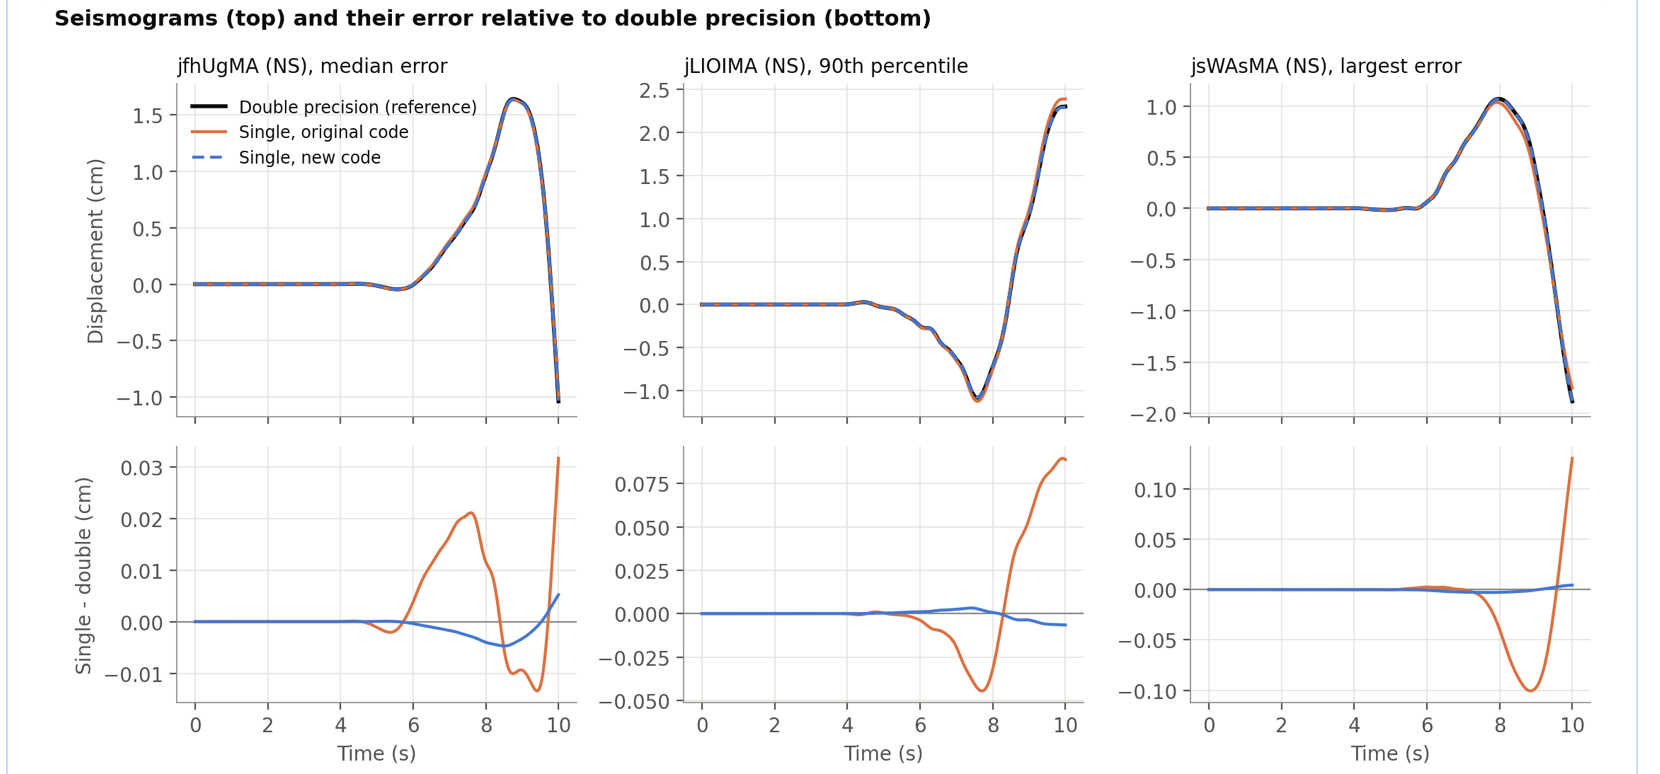
\includegraphics[width=\textwidth]{figures/source_trim_accuracy.png}
  \caption{Station seismograms (top) and their error relative to double
    precision (bottom) for three stations of the \code{input\_k4} rupture
    case: original single-precision code (orange) and with trimmed source
    splines (blue).}
  \label{fig:srcacc}
\end{figure}

\section{Build configuration}
\label{sec:build}

\subsection{Portability}
The CMake build was extended to work with the Mahuika toolchains
(\code{gimkl}, \code{intel}, \code{foss}, AOCC with OpenMPI) (PR~\pr{3}). This
required restricting the MPI search to C/C++ (AOCC's \code{flang} cannot read
\code{gfortran} module files), a configurable number of OpenMP threads per test
to avoid oversubscription, and an \code{hpc3-genoa} target that falls back to
\code{znver3}+AVX-512 when the compiler lacks \code{znver4}. Further changes
switched the build to C++17 (PR~\pr{6}), removed redundant \code{\#pragma ivdep}
next to \code{\#pragma omp simd} that broke oneAPI builds (PR~\pr{17}), and
made CMake require a parallel HDF5 when \code{USE\_HDF5=ON} (PR~\pr{31}).

\subsection{Compiler and target comparison}
Fig.~\ref{fig:compilers} compares toolchains on \code{gausshill-att-3}.
Initially (generic targets) Intel was fastest on most tests, \code{gimkl}
1.0--1.45$\times$ slower and AOCC 1.4--2.1$\times$ slower, with the largest
gaps on tests with attenuation. Targeting the Genoa architecture improved the
Intel build by $\sim$1.2$\times$, mostly in the curvilinear stencil
(\code{curvilinear4sg}, 1.45$\times$ from SSE2 to AVX2).

\begin{figure}[ht]
  \centering
  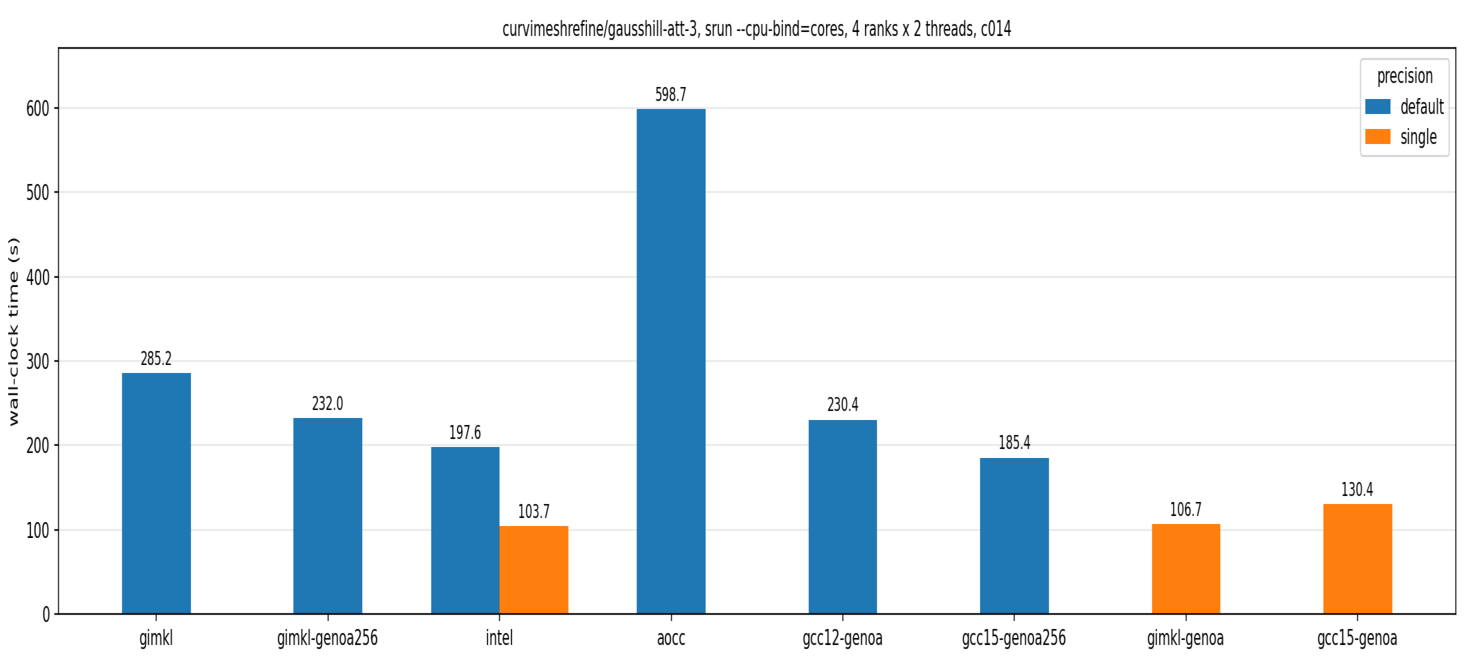
\includegraphics[width=\textwidth]{figures/compiler_comparison_gausshill.png}
  \caption{Wall-clock time of \code{gausshill-att-3} for different toolchains
    and targets (4 ranks $\times$ 2 threads, Genoa node).}
  \label{fig:compilers}
\end{figure}

The decisive step was enabling 512-bit vectors with the classic Intel compiler.
Zen~4 implements a subset of AVX-512 which \code{-march=icelake-server}
targets; \code{-qoverride-limits} is needed to stop the compiler giving up on
4 of the 5 loops in \code{curvilinear4sg\_ci\_impl}, and
\code{-qopt-zmm-usage=high} to use full-width registers. Table~\ref{tab:intel}
shows the resulting single-precision timings.

\begin{table}[ht]
  \centering
  \caption{\code{gausshill-att-3}, single precision, 4 ranks $\times$ 2 threads,
    4 runs per build on the same Genoa node (range in brackets).}
  \label{tab:intel}
  \begin{tabular}{lccc}
    \toprule
    build & time stepping (s) & wall (s) & wall vs Intel \\
    \midrule
    Intel \code{icpc}, AVX-512 & 71.3 (69.2--73.2) & 82.8 (79.1--85.1) & -- \\
    GCC 15.2, \code{-march=znver4}, 512-bit & 101.3 (100.5--102.3) & 104.9 & +27\% \\
    GCC 15.2, \code{-march=znver4}, 256-bit & 99.2 (97.8--101.4) & 106.8 & +29\% \\
    \bottomrule
  \end{tabular}
\end{table}

For comparison, the same case took over 200~s with \code{gimkl} and about
360~s with AOCC. The recommended build is
\begin{lstlisting}
module purge; module load intel/2022a
cmake -DCMAKE_BUILD_TYPE=Release -DBUILD_SW4MOPT=OFF \
      -DCMAKE_C_COMPILER=mpiicc -DCMAKE_CXX_COMPILER=mpiicpc \
      -DCMAKE_Fortran_COMPILER=ifort \
      -DSW4_TARGET=hpc3-genoa -DUSE_DOUBLE=OFF ..
\end{lstlisting}

\paragraph{oneAPI container.} SW4 was also built with Intel oneAPI
(\code{icpx}) inside an Apptainer container. With controlled pinning, the
container build runs at the same speed as the native \code{icpc} build
(ratio 1.002 on \code{lamb-3}, 450.8 versus 449.7~s), with the same accuracy.
Apparent gaps of 5--33\% seen earlier were caused by rank placement, not by the
compiler or the container.

\section{Profiling infrastructure}
\label{sec:timers}

Profiling with TAU on Mahuika was used in the first weeks. To make profiling
routine for the researchers, hierarchical region timers were added directly to
SW4 (PRs~\pr{36}, \pr{37}):
\begin{itemize}[itemsep=0pt]
  \item \code{SW4\_TIME("name")} scoped timers for the main phases, the
        predictor/corrector sub-steps, output, \code{enforceIC} and the
        interface solve, and each attenuation mechanism in \code{evalRHS};
  \item an end-of-run table of min/avg/max over ranks, optionally written as
        CSV (\code{SW4\_TIMERS\_CSV});
  \item PMPI wrappers that charge MPI time, bytes and messages to the
        innermost region (CMake option \code{SW4\_TIMERS\_MPI});
  \item an OMPT tool that measures per-thread busy time and therefore OpenMP
        load imbalance and fork/join overhead.
\end{itemize}
The timers revealed, for example, that \code{enforceIC} launched about 180 small
parallel regions per time step with 77--86\% thread idle time, and that the
forcing dominated the rupture-source cases. They were used to produce the
phase breakdowns in Section~\ref{sec:scaling}.

\section{Performance optimisations}
\label{sec:opt}

Table~\ref{tab:opt} lists the code optimisations. All are bit-identical to the
code they replace unless stated otherwise.

\begin{table}[ht]
  \centering
  \caption{Code optimisations. Speedups are for the stated region or case.}
  \label{tab:opt}
  \small
  \begin{tabularx}{\textwidth}{lX>{\raggedright\arraybackslash}p{5.5cm}}
    \toprule
    PR & change & effect \\
    \midrule
    \pr{5} & \code{Sarray::assign}: loop over $(k,j)$ then $i$ when reordering a Fortran-order array & part of \code{lamb-3}: 1026 $\to$ 431~s \\
    \pr{7} & \code{rhs4th3fort(sgstr)\_ci}: zero only the halo of \code{lu}, not the whole array & fewer memory sweeps \\
    \pr{14} & Cartesian RHS kernels: tile the interior loop in $j$ so the $k$-stencil stays in L2 & Cartesian RHS \\
    \pr{13} & Exact Lamb solution evaluated on the surface plane only & faster Lamb tests \\
    \pr{34} & Pass grid point source vectors by \code{const} reference (were copied every call) & forcing \\
    \pr{41}$^\dagger$ & Evaluate each distinct source time function once per \code{Force}/\code{Force\_tt} call & \code{input\_k4}: 66~min $\to$ 40~min (1.65$\times$), memory 19.4 $\to$ 16.4~GB \\
    \pr{38} & Constant-bound loops in the upper SBP closure of the curvilinear and anisotropic kernels & curvilinear RHS 2.3$\times$; \code{k4\_c8} 1.8$\times$ \\
    \bottomrule
  \end{tabularx}
  \\[0.3em]
  {\footnotesize $^\dagger$ Merged by J.~Faulkner, combining the cache
  (commits \code{0140da08}, \code{8780d28e}) with tabulation of the
  prefiltered time functions.}
\end{table}

\paragraph{Source time-function cache.}
QuakeCore's rupture models contain tens of thousands of subfault sources which
are distributed to millions of grid-point sources, but only about one in a
hundred has a distinct time function. Evaluating each distinct function once
per call reduced the forcing on the \code{input\_k4} case from 318~s to 2.5~s.
In production, the QuakeCore team reported that this optimisation reduced the run time of the
Darfield campaign (162 runs, some on curvilinear grids) from about 3~h to
1.5~h per run, as the forcing on the ranks overlapping the fault was holding
up all other ranks.

\paragraph{Upper SBP closure.}
The curvilinear stencil's upper boundary closure ($k=n_k-5,\dots,n_k$) ran
4.5$\times$ slower per point than the lower closure because its inner loops
had run-time bounds (\code{q = nk-7 .. nk}), which prevented the compiler from
unrolling and vectorising them efficiently. Rewriting them with constant trip
counts made both closures equally fast. Because QuakeCore's curvilinear grids
are thin (13--14 planes), the closure covers $\sim$45\% of the curvilinear
points, so the curvilinear RHS dropped from 38.1 to 16.8~s and the
\code{k4\_c8} test case from 113.9 to 63.1~s.

\paragraph{Work not (yet) merged.}
\begin{itemize}[itemsep=0pt]
  \item \emph{Fused attenuation mechanisms} (branch
    \code{fuse-attenuation-mechanisms}): one sweep for all attenuation
    mechanisms in the curvilinear RHS. Bit-identical, but only 4.6\% faster,
    since that kernel is compute bound.
  \item \emph{Merged interface Jacobi kernels} (branch
    \code{enforceic-jacobi-merge}): the four Jacobi kernels in \code{consintp}
    run in a single parallel region. Jacobi $-45\%$, \code{enforceIC}
    $-23\%$, time step $\sim-3\%$. Also fixes the residual bug below.
  \item \emph{Shorter prefilter precursor} (\code{precursor\_efolds} option):
    8 instead of 12 e-folds saves 21\% of time steps, but changes weak traces
    by up to 40\%. The plan, currently, is to keep the precursor but at the same time
    investigate filtering as a post-processing step.
\end{itemize}

\section{Bug fixes}
\label{sec:bugs}
\begin{itemize}[itemsep=2pt]
  \item \textbf{Parallel I/O} (PR~\pr{35}): the chunked float read and write
        paths in \code{Parallel\_IO} were broken for large single-precision
        transfers.
  \item \textbf{Interface Jacobi residual}: the \code{omp simd} loops updated
        the max-norm residual without a reduction clause (undefined behaviour),
        giving a wrong residual on multiple ranks. Fixed on
        \code{enforceic-jacobi-merge}.
  \item \textbf{Tests}: the old unit tests were reinstated
        (\code{ctest -L unit}) and the \code{lamb-1} and attenuation reference
        files regenerated (PRs~\pr{12}, \pr{32}).
\end{itemize}

\section{Runtime configuration and scaling}
\label{sec:scaling}

\subsection{Process binding}
Many apparent performance differences early in the project were caused by rank
placement rather than by the code. The recommended settings with Slurm are
\begin{lstlisting}
export OMP_NUM_THREADS=${SLURM_CPUS_PER_TASK}
export OMP_PROC_BIND=close
export OMP_PLACES=cores
srun --mpi=pmix --cpu-bind=cores sw4 input.in
\end{lstlisting}
(\code{--mpi=pmi2} for Intel MPI and OpenMPI~4). With OpenMPI and
\code{mpiexec}, \code{--map-by slot:PE=N --bind-to core} is required, otherwise
ranks are left unbound and threads pile up on the same cores.

\subsection{MPI/OpenMP balance}
On a 64-core Cascade allocation (\code{small} case, 242 steps), the time
stepping is 23--30\% slower with pure MPI (64$\times$1) than with 2--8 threads
per rank; 16$\times$4 is fastest, within 5\% of 32$\times$2 and 8$\times$8.
For short runs, however, a phase outside time stepping grows as the number of
ranks decreases, so total wall time favours fewer threads.

On full Cascade nodes (2 sockets, 24 CCDs of 8 cores sharing an L3 cache),
the best layout is one rank per CCD, i.e.\ 24 ranks $\times$ 8 threads per
node, with every rank's threads confined to its CCD
(Table~\ref{tab:layout}). SW4 is memory bound, and hyperthreading makes it
31\% slower.

\begin{table}[ht]
  \centering
  \caption{Rank/thread layouts on 8 Cascade nodes (351~M grid points, 4166 steps).}
  \label{tab:layout}
  \begin{tabular}{lrrrr}
    \toprule
    layout per node & ranks & time stepping (s) & ns/point/step/node & vs 24$\times$8 \\
    \midrule
    24 $\times$ 8 & 192 & 1879.8 & 10.28 & -- \\
    24 $\times$ 16, hyperthreads & 192 & 2458.0 & 13.44 & +31\% \\
    48 $\times$ 4 & 384 & 1922.6 & 10.51 & +2.3\% \\
    \bottomrule
  \end{tabular}
\end{table}

\subsection{Strong and weak scaling}
Strong scaling on one Cascade node (\code{input\_k4\_c4}, 2 threads per rank)
gives a speedup of 2.96 going from 6 to 24 ranks (74\% efficiency).

For weak scaling the grid spacing was refined from 800~m to 400~m so that each
node holds about 44~M grid points, from 1 to 8 nodes (192 ranks, 1536 cores).
The time per grid point per step per node falls from 11.33 to 10.28~ns, an
efficiency of 1.10 (Fig.~\ref{fig:weak}). The solver alone has an efficiency
of 1.05. Efficiency exceeds 1 because some work does not grow with the node
count: the rupture source has a fixed number of subfaults and the surface
images grow with area rather than volume. Communication stays at about 17\% of
the step time at all node counts, half of which is waiting for slower ranks.
The largest remaining imbalance is in the forcing: at 8 nodes the busiest rank
spends about 43$\times$ the average time on it, since only ranks overlapping the
fault do source work.

\begin{figure}[ht]
  \centering
  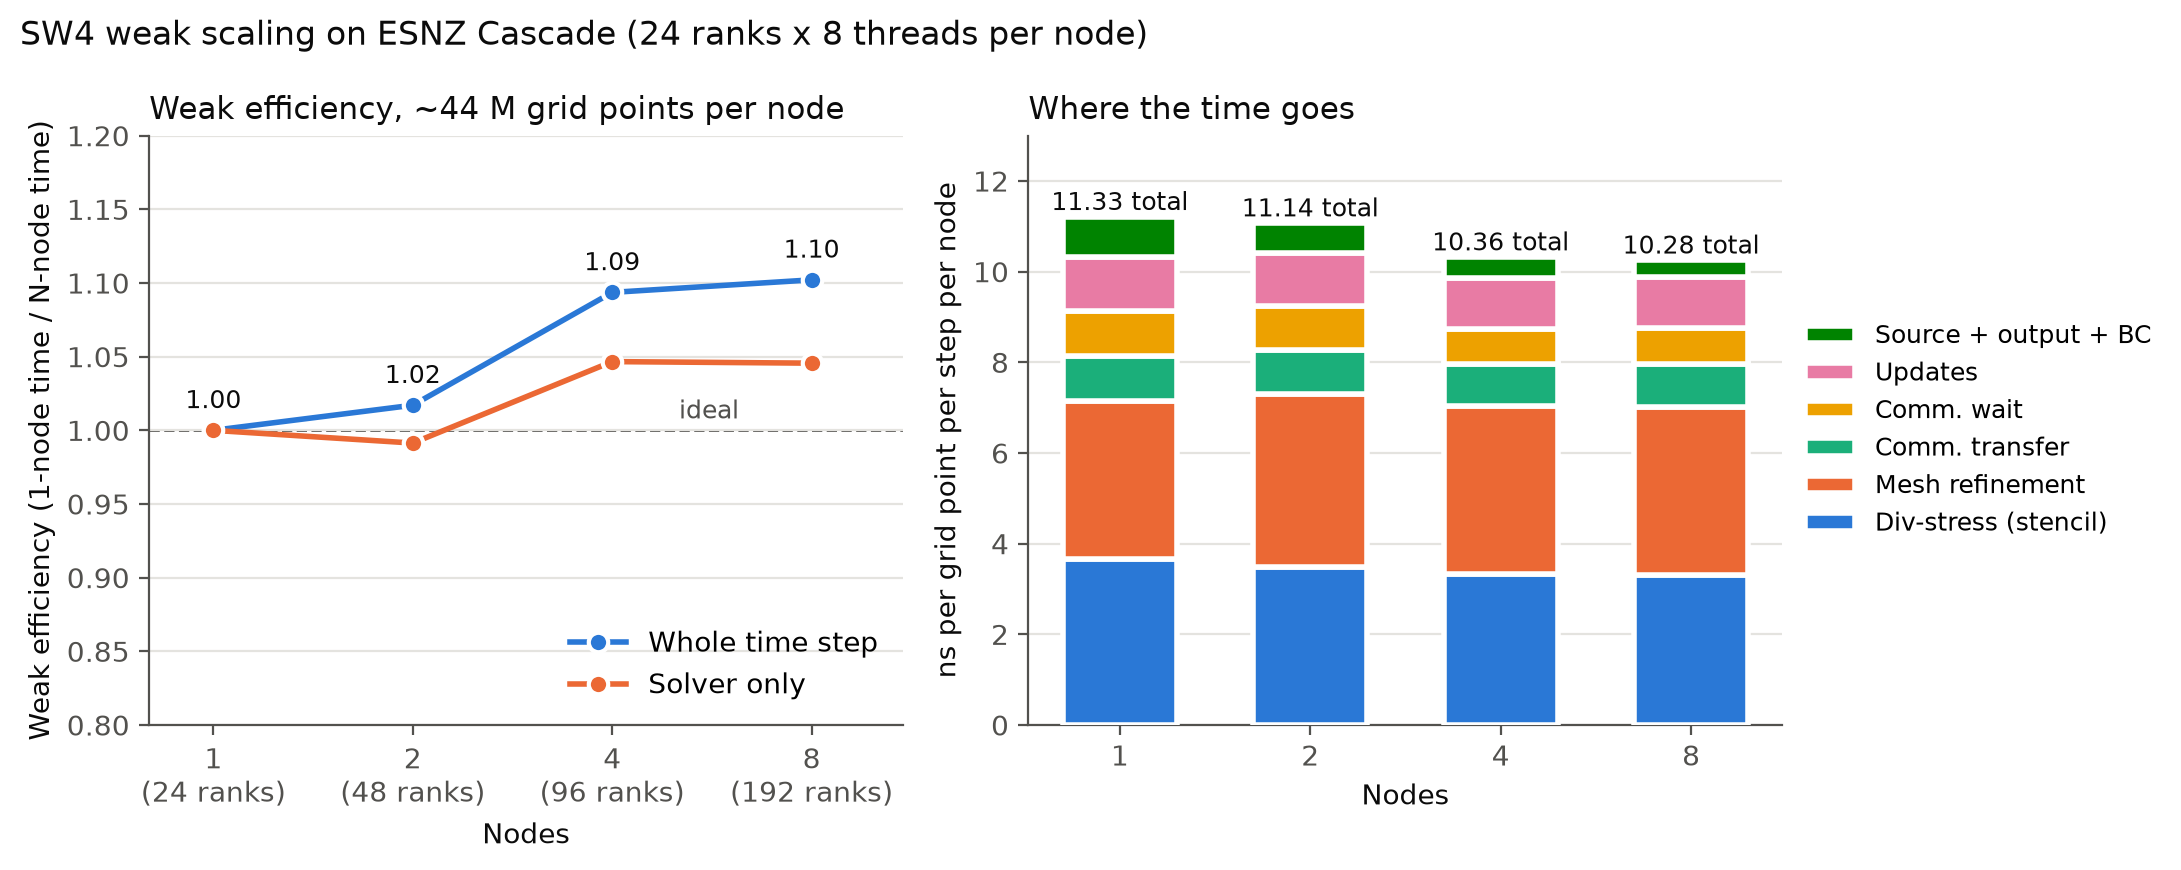
\includegraphics[width=\textwidth]{figures/weak_scaling_cascade.png}
  \caption{Weak scaling of SW4 on Cascade, 24 ranks $\times$ 8 threads per node.
    Left: efficiency of the whole time step and of the solver alone. Right:
    time per grid point per step per node by phase.}
  \label{fig:weak}
\end{figure}

\section{Pull requests merged upstream}

\begin{table}[ht]
  \centering
  \small
  \begin{tabularx}{\textwidth}{llX}
    \toprule
    PR & merged & description \\
    \midrule
    \pr{2}  & 30 Sep & Single-precision build fixes (Clang 21, \code{pow} promotion), test tolerances \\
    \pr{3}  & 30 Sep & Multi-toolchain CMake build on Mahuika, AVX-512 flags for \code{icpc} on Genoa \\
    \pr{5}  & 1 Oct  & \code{Sarray::assign} loop reordering \\
    \pr{6}  & 5 Oct  & Build with C++17 \\
    \pr{7}  & 8 Oct  & Zero only the halo in \code{rhs4th3fort(sgstr)\_ci} \\
    \pr{12} & 8 Oct  & Regenerate attenuation reference files \\
    \pr{13} & 8 Oct  & Exact Lamb solution on the surface plane only \\
    \pr{14} & 8 Oct  & $j$-tiling of the Cartesian RHS kernels \\
    \pr{17} & 9 Oct  & Remove \code{\#pragma ivdep} next to \code{\#pragma omp simd} \\
    \pr{31} & 9 Oct  & CMake: require a parallel HDF5 \\
    \pr{32} & 12 Oct & Reinstate unit tests (\code{ctest -L unit}) \\
    \pr{34} & 13 Oct & Pass point-source vectors by \code{const} reference \\
    \pr{36} & 14 Oct & Hierarchical region timers, MPI and OMPT profiling \\
    \pr{35} & 16 Oct & \code{Parallel\_IO} chunked float read/write fix \\
    \pr{37} & 16 Oct & Pre-roll progress; per-mechanism attenuation timers \\
    \pr{38} & 16 Oct & Constant-bound loops in the upper SBP closure \\
    \bottomrule
  \end{tabularx}
\end{table}
In addition, the source time-function cache was merged as part of
PR~\pr{41} (16 Oct).

\section{Next steps}
\begin{itemize}[itemsep=2pt]
  \item Contribute some or all of the enhancements back to the original SW4
        code (\href{https://github.com/geodynamics/sw4}{\code{geodynamics/sw4}}),
        so that the wider SW4 community benefits and QuakeCore's fork does not
        drift further from upstream. Candidates include the build portability
        fixes, the region timers, the bug fixes, and the precision-independent
        kernel optimisations (SBP closure, source time-function cache,
        \code{Sarray::assign}, RHS tiling).
  \item Open pull requests for the merged interface Jacobi kernels (with the
        residual fix) and decide on the fused attenuation kernel.
  \item Investigate the decomposition of irregular domains such as the
        Darfield model, and map the domain decomposition onto the CCD layout.
  \item Reduce the forcing imbalance on ranks overlapping the fault.
  \item Vectorise the anisotropic curvilinear kernels, which currently do not
        vectorise at all.
  \item Reduce start-up and output cost (HDF5 paging already reduced start-up
        from 30 to 1~min on one case).
  \item Repeat the scaling study on the Darfield input and on CyberShake-size
        sources.
\end{itemize}

\end{document}
